\documentclass{beamer}

\usepackage{subfigure}
\usepackage{graphicx}
\usepackage{sidecap}
\usepackage{caption}
%\usepackage{subcaption}
\captionsetup{compatibility=false}
\usepackage{appendixnumberbeamer}
\usepackage{amsmath}
% --
\usepackage{multirow}
\usepackage{xcolor}
\usepackage{setspace}
\usepackage{hyperref}
\usepackage{anyfontsize}

\beamertemplatenavigationsymbolsempty
\setbeamertemplate{footline}

\newenvironment{itemise} {\begin{itemize} \setlength{\itemsep}{0.2cm}} {\end{itemize}}
\usepackage[labelformat=empty]{caption}
\setbeamertemplate{sections/subsections in toc}[square]

%% COLORS
\definecolor{Gray}{gray}{0.9}
\definecolor{dblue}{rgb}{0.132,0.1,0.27}
\definecolor{mint}{cmyk}{1.0, 0.2, 0.6, 0.05}
\definecolor{ant}{cmyk}{0.5, 0.1, 0.0, 0.45}
\definecolor{lgray}{cmyk}{0.12, 0.0, 0.0, 0.17}
\definecolor{lred}{cmyk}{0.0, 0.9, 0.7, 0.0}


\usepackage{etoolbox}% http://ctan.org/pkg/etoolbox 
\usepackage{booktabs}

\newenvironment{literatur}{%
  \parskip2pt \parindent0pt \raggedright
  \def\lititem{\hangindent=0.5cm \hangafter1}}{%
  \par\ignorespaces}


\newcommand{\tb}[1]{{\color{blue}{\textbf{#1}}}}
\newcommand{\tm}[1]{{\color{mint}{\textbf{#1}}}}
\newcommand{\tr}[1]{{\color{red}{\textbf{#1}}}}
\newcommand{\tbs}[1]{{\color{blue}{#1}}}
\newcommand{\trs}[1]{{\color{red}{#1}}}
\newcommand{\tms}[1]{{\color{mint}{#1}}}
\newcommand{\tps}[1]{{\color{purple}{#1}}}
% Ilya: packages

\usepackage{tikz}
\usepackage{lmodern}
\usepackage{enumitem}

% Ilya: my commands

\newenvironment{mytemize}
{\vfill\itemize[nolistsep,itemsep=\fill,label=\color{blue}{$\triangleright$}]}
  {\enditemize}


\newenvironment{mynumerate}
{\vfill\enumerate[nolistsep,itemsep=\fill,label=\arabic*.]}
  {\endenumerate}

\newcommand{\hitem}[1]{
  {\color{blue}{$\triangleright$}} 
  {#1} 
  {\hfill}
}

\setlist[itemize]{label= \color{blue}{$\triangleright$}}
\setlist[enumerate]{label = \arabic*.}

\newcommand{\rarr}{$\Rightarrow$\ }



%\href{<Ziel>}{<Eingefasster Text>} 

%\logo{\includegraphics[height=0.7cm]{BdFlogo.eps}\hspace{300pt}\vspace{-5pt}}
%\logo{\includegraphics[height=0.8cm]{BdFlogo.eps}}
%\logo{\pgfputat{\pgfxy(-6.2,-0.5)}{\pgfbox[center,base]{\includegraphics[height=0.8cm]{BdFlogo.eps}}}}

%------------------------------------------------------------------------------------
% TITLE
%------------------------------------------------------------------------------------
\title[PSME]{Macroeconomics\\ Lecture 7 -- Real Business Cycles in Closed Economy} 
\author[I. Eryzhenskiy]{Ilya Eryzhenskiy}
\institute[BdF]{PSME Panth\'{e}on-Sorbonne Master in Economics}
\date[PSME macro]{Fall 2023}

%---BEGIN------------------------------------------------------------------------------
\begin{document}

\begin{frame}
  \maketitle
\end{frame}

\begin{frame}{Overview}
  \tableofcontents
\end{frame}


%---FRAME------------------------------------------------------------------------------
\section{Representative household}
%---FRAME------------------------------------------------------------------------------
\begin{frame}
\frametitle{Outline}
\tableofcontents[currentsection]
\end{frame}

\begin{frame}{Representative household}

  A \textbf{large number} (population size normalized to 1) of \textbf{identical} households populate the economy. 
  \vfill
  A \tb{representative household}: the aggregate outcomes as result of one (big) agent's behaviour.
  \vfill 
  It represents many small ones \rarr the representative household cannot manipulate aggregate quantities and prices (wage, interest) \rarr \textbf{takes prices as given}
  \vfill
  Households in RBC model \textbf{live forever}:
  \begin{mytemize}
  \item Demographics ignored (unlike overlapping generations models)
  \item Imagine a sequence of generations of constant size
	, with children' utility entering parents' utility
  \end{mytemize}
\end{frame}
%---FRAME------------------------------------------------------------------------------
\begin{frame}{Representative household -- budget constraint} 
Household chooses work effort and earns wage $w_t$, but also has several types of financial income:
\begin{mynumerate}
    \item it invests in bonds: $B_{t+1}$ is the the stock of bonds at held \trs{at the beginning of $t+1$}, which is \trs{chosen in $t$}. It pays the \trs{real interest rate $r_t$ in $t+1$}
    \item it invests in physical capital: $K_{t+1}$ is the stock at \trs{beginning of $t+1$}, that is result of investment in $t$, $I_t$. Capital depreciates at rate $\delta$: $$K_{t+1} = (1-\delta)K_{t} + I_t$$ 
    capital is \textbf{rented out to firms}, and in period $t$ the stock of capital $K_t$ pays the \tb{rental rate of capital} $R_t$ to the household%. In practice, $K_{t+1}$ is used as choice variable of household, not $I_t$
    \item it owns the firms \rarr receives their profits $\Pi_t$
\end{mynumerate}
\end{frame}
%---FRAME------------------------------------------------------------------------------

\begin{frame}{Representative household budget}
The household budget constraint is then:

$$
C_t+\underbrace{K_{t+1}-(1-\delta) K_t}_{I_t}+\underbrace{B_{t+1}-B_t}_{\text{bond saving}}=w_t N_t+R_t K_t+r_{t-1} B_t+\Pi_t
$$
re-arranging terms, we get:
$$
C_t+K_{t+1}+B_{t+1}=w_t N_t+(R_t+1-\delta) K_t +(1+r_{t-1}) B_t+\Pi_t
$$

The convention about stock variables $K, B$ here is \textbf{measuring stock variables at the beginning of period}. 

Difference between bonds and capital as sources of income: 
\begin{itemize}
    \item  the real interest rate is known one period in advance before it is paid on bonds ($r_{t-1}$ on $B_t$, $r_t$ on $B_{t+1}$)
    \item rental rate of capital is determined at the same period when it is paid: the household does not know it in advance when investing in capital ($R_{t+1}$ paid on $K_{t+1}$ that is chosen in $t$)
\end{itemize}

\end{frame}

\begin{frame}{Representative household maximization problem}
    We will make an additional assumption for the instantaneous utility function: it is \tb{additively separable} between consumption and leisure utility:
    $$u(C_t, 1-N_t) = u(C_t)+v(1-N_t)$$
    We can now write the household problem with infinite horizon:
   \begin{align*}
&\max _{C_t, N_t, K_{t+1}, B_{t+1}} E_0 \sum_{t=0}^{\infty} \beta^t\left(u\left(C_t\right)+v\left(1-N_t\right)\right) \\
\text{s.t.}\ C_t+&K_{t+1}+B_{t+1}=w_t N_t+(R_t+1-\delta) K_t +(1+r_{t-1}) B_t+\Pi_t
\end{align*}
\end{frame}

%---FRAME------------------------------------------------------------------------------

\begin{frame}{Household problem: solution}

Lagrangian of household problem
\begin{align*}
\mathcal{L} = E_0 \sum_{t=0}^{\infty} \beta^t 
[  u(C_t&) + v(1-N_t) \\
+ \lambda_t &\left( w_t N_t+(R_t+1-\delta) K_t\right. +(1+r_{t-1}) B_t+\Pi_t \\  &-C_t - K_{t+1} - \left.B_{t+1}\right)]
\end{align*}
First-order conditions in period $t$ \tms{(with information of $t$ \rarr $E_t[\cdot]$):}
\begin{align*}
&(1) \quad \frac{\partial \mathcal{L}}{\partial C_t}: \quad &  &u'(C_t)-\lambda_t = 0\\
&(2) \quad \frac{\partial \mathcal{L}}{\partial N_t} : \quad &  &-v'(1-N_t)+ \lambda_t w_t=0\\
&(3) \quad \frac{\partial \mathcal{L}}{\partial B_{t+1}} : \quad &  &-\lambda_t +\beta E_t\lambda_{t+1}(1+r_{t})=0 \\
&(4) \quad \frac{\partial \mathcal{L}}{\partial K_{t+1}} : \quad &  &-\lambda_t +\beta E_t[\lambda_{t+1}(R_{t+1} + 1 - \delta)]=0 
\end{align*}

\end{frame}
%---FRAME------------------------------------------------------------------------------
\begin{frame}{Household problem: solution}

\begin{mytemize}
\item From $\frac{\partial \mathcal{L}}{\partial C_t}=0$ and $\frac{\partial \mathcal{L}}{\partial N_t}=0$, \tb{consumption-leisure optimality} or labor supply conditional on consumption level: $$\frac{v'(1-N_t)}{u'(C_t)} = w_t, \text{\ or}\ N_t = N^s(w_t, C_t)$$ \tms{$\frac{v'(1-N_t)}{u'(C_t)}$ is $\frac{-u'_L(C_t, 1-N_t)}{u'_C(C_t,1-N_t)}$ in previous notation}
\item From $\frac{\partial \mathcal{L}}{\partial C_t}=0$ and $\frac{\partial \mathcal{L}}{\partial B_t}=0$, the  \tb{Euler equation}: $$u'(C_t) = \beta E_t u'(C_{t+1})(1+r_t)$$ 
\item From $\frac{\partial \mathcal{L}}{\partial C_t}=0$ and $\frac{\partial \mathcal{L}}{\partial K_t}=0$, \tb{capital holding optimality}: $$u'(C_t) = \beta E_t [u'(C_{t+1})(R_{t+1}+1-\delta)]$$ 
where $E_t$ applies to product of $u'(C_{t+1})$ and $R_{t+1}$, both uncertain, and $E(XY) \neq E(X)E(Y)$ in general, so we \tr{cannot conclude that $r_t = E_t R_{t+1}-\delta$!}
\end{mytemize}
\end{frame}
%---FRAME------------------------------------------------------------------------------
\begin{frame}{Euler equation and Stochastic Discount Factor}

Define the \tb{stochastic discount factor} $M_t$ as $$M_t =  \frac{\beta^t E_0  u'(C_t)}{u'(C_0)}$$
    Multiplying uncertain future income in period $t$ by $M_t$ gives its \textbf{present discounted value} \vfill
    Why? Use the \tb{Euler equation}:
    \begin{align*}
    u'(C_t) = \beta E_t u'(C_{t+1})(1+r_t) &\Leftrightarrow \frac{u'(C_t)}{\beta E_t u'(C_{t_1})} = 1+r_t \\&\Leftrightarrow \frac{\beta E_t u'(C_{t+1})}{u'(C_{t})} = \frac{1}{1+r_t}
    \end{align*}
    and:
    \begin{align*}
    M_t &=  \frac{\beta^t E_0 u'(C_t)}{u'(C_0)} =   E_0  [ \underbrace{\frac{\beta u'(C_1)}{u'(C_0)}}_{1/(1+r_0)}\cdot \underbrace{\frac{\beta u'(C_2)}{u'(C_1)}}_{1/(1+r_1)}\dots  \underbrace{\frac{\beta u'(C_t)}{u'(C_{t-1})}}_{1/(1+r_{t-1})} ]  \\
    &= \frac{1}{1+r_0}\cdot E_0 \left[ \frac{1}{1+r_1} \frac{1}{1+r_2}\dots \frac{1}{1+r_{t-1}} \right] \tms{=E_0 \frac{1}{R_{0,t}} \text{\ (see Lec. 5)}}
    \end{align*}
\end{frame}
%---FRAME------------------------------------------------------------------------------

%---FRAME------------------------------------------------------------------------------
\section{Representative firm}
%---FRAME------------------------------------------------------------------------------
\begin{frame}
\frametitle{Outline}
\tableofcontents[currentsubsection]
\end{frame}
%---FRAME------------------------------------------------------------------------------
\begin{frame}{Representative firm}

  A continuum of small, identical firms  \rarr study \tb{representative firm} \vfill
  Production function $A_t F(K_t, N_t)$ with \tb{constant returns to scale} and TFP $A_t$ that is \textbf{known at beginning of $t$}
\vfill
Maximize present discounted value of profits:
  \begin{itemize}
\item[] Revenue from production ($=$ production because $P=1$) 
\item[$-$] Cost of production: wage for labor, rental rate for capital
  \end{itemize}
\vfill
\tb{Perfect competition} \rarr firms takes factor prices $w_t, R_t$ as given
\vfill
Firm choices turn out to be static, i.e. solving a one-period problem is enough
\vfill
\tms{In the textbook, read section 2.2 Households own capital stock and ignore debt variable $D_t$ that is shown to be neutral}
\end{frame}
%---FRAME------------------------------------------------------------------------------
\begin{frame}{Firm profit maximization}

  Maximize discounted future profits ($=$ firm value):
\begin{align*}
V_0 = \sum_{t=0}^{\infty} M_t \Pi_t =  \sum_{t=0}^{\infty} M_t \left( A_t F(K_t,N_t)-w_t N_t - R_t K_t \right)
\end{align*}
Where households' stochastic discount factor $M_t$ is used because households are firm owners \vfill
Every period $t$ has variables $t$ only \rarr firm problem is static:
$\max_{N_t,K_t} A_t F(K_t,N_t)-w_t N_t-R_t K_t$ \vfill
First-order conditions:
\begin{align*}
K_t: \quad \quad A_t F'_K(K_t,N_t)-R_t &= 0 \ \rarr K_t = K^d(A_t, R_t)\\
N_t: \quad \quad A_t F'_N(K_t,N_t)-w_t &= 0 \ \rarr N_t = N^d(A_t, w_t)
\end{align*}
FOCs define a \tb{capital demand function} $K^d(A_t, R_t)$ and a \tb{labor demand function} $N^d(A_t, w_t)$ \\
Perfect competition, constant returns to scale \rarr $\Pi_t = 0$
\end{frame}
%---FRAME------------------------------------------------------------------------------
%---FRAME------------------------------------------------------------------------------
\section{Equilibrium}
%---FRAME------------------------------------------------------------------------------
\begin{frame}
\frametitle{Outline}
\tableofcontents[currentsubsection]
\end{frame}
%---FRAME------------------------------------------------------------------------------
\begin{frame}{Dynamic equilibrium: diagram}
\begin{center}
%{\small
%Figure. 
%}
\vspace{-5mm}
\begin{figure}[h!]
	\subfigure{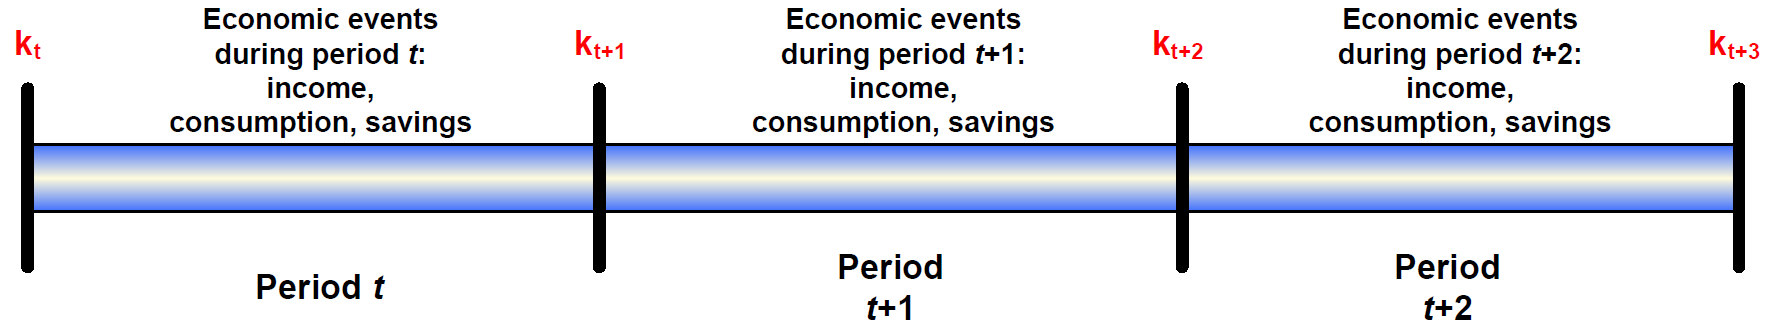
\includegraphics[trim=0 0 0 0,clip,width=1.1\textwidth]{FIGURES/10_Time_cropped}
	}      
	%\subfigure{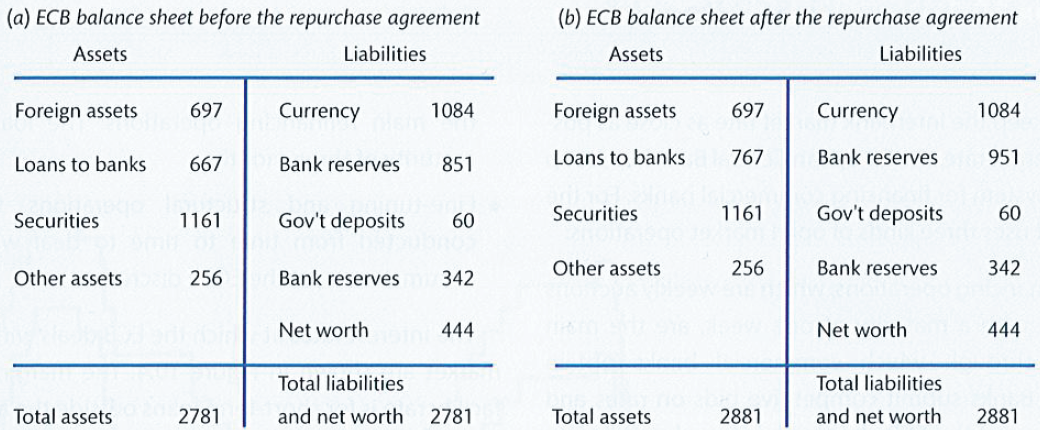
\includegraphics[trim=0 00 0 00,clip,width=0.6\textwidth]{FIGURES/5_CB_balance_sheet_OMO}
	%} 	
	%[trim=left bottom right top
\end{figure}
%\vspace{-2mm}
%\begin{minipage}{0.5\columnwidth}
%\tiny	
%\textbf{Source.} Burda and Wyplosz (2017), Figure 14.1.\\
%\end{minipage}
\end{center}
\end{frame}


\begin{frame}{Market clearing conditions}
  \textbf{Capital market clearing} \\
  \begin{mytemize}
  \item Capital demand from firm's profit maximization: $K_{t} = K^d(A_{t}, R_{t})$
  \item Capital supply is given by HH's consumption-saving decisions: $K_{t} = K^s(C_{t-1}, E_{t-1} C_{t}, E_{t-1} R_t)$
  \item Combining:
  $K_t = K^d(A_{t}, R_{t})=K^s(C_{t-1}, E_{t-1} C_{t}, E_{t-1} R_t)$
  \end{mytemize}
\vfill
\textbf{Goods market clearing}
\begin{mytemize}
\item Goods supply, or GDP, is $Y_t = A_t F(K_t,N_t)$
\item Goods demand is $C_t+I_t$, with $I_t= K_{t+1} - (1-\delta)K_{t}$ 
\item Combining: $C_t+K_{t+1}-(1-\delta)K_{t}=A_t F(K_t,N_t)$ \\ \rarr \tb{aggregate resource constraint}
\end{mytemize}
\vfill
\textbf{Labor market clearing}: $N^s(w_t, C_t) = N^d(A_t, w_t)$ \vfill
\textbf{Bond market clearing}: $B_t = 0$ since all households are the same (no borrowers, no savers)
\end{frame}
%---FRAME------------------------------------------------------------------------------
\begin{frame}{Dynamic equilibrium: definition}

A dynamic equilibrium is a sequence $\left\{ C_t,N_t, K_{t},B_{t},w_t,r_t,R_t,\right\}_{t=0}^{\infty}$ that, given exogenous initial capital $K_0>0$ and bonds $B_0=0$ and the exogenous stochastic processes for $\{A_t\}_{t=0}^\infty$, satisfies:
\begin{mynumerate}
\item Given $\left\{ w_t, r_t, R_t\right\}_{t=0}^{\infty}$, $\left\{ C_t, N_t,K_{t+1},B_{t+1}\right\}_{t=0}^{\infty}$ satisfies the sequence of consumption-leisure optimality conditions, consumption-saving optimality conditions, and consumer budget constraints
\item Given $\left\{w_t, R_t \right\}_{t=0}^{\infty}$, $\left\{ N_t,K_t\right\}_{t=0}^{\infty}$ satisfies the sequence of labor demand functions and capital demand functions
\item All markets clear: $Y_t = C_t+K_{t+1}-(1-\delta)K_{t}=A_t F(K_t,N_t)$; $N^s_t=N^d_t=N_t$; $K^s_t=K^d_t=K_t$, $B_t = 0$
\end{mynumerate}

\end{frame}
%---FRAME------------------------------------------------------------------------------
\begin{frame}{Dynamic equilibrium: system of equations}
At each $t\geq 0$, $(C_t,N_t, K_{t},w_t,r_t,R_t,A_t)$
satisfies
\begin{align*}
\frac{v'(1-N_t)}{u'(C_t)}&= w_t \nonumber\\
u'(C_t) &= \beta E_t u'(C_{t+1})(1+r_t) \\
u'(C_t) &= \beta E_t [u'(C_{t+1})(R_{t+1}+1-\delta)] \\
 A_t F'_N(K_t,N_t) &= w_t \nonumber\\
 A_t F'_K(K_t,N_t) &= R_t \nonumber\\
C_t+K_{t+1}-(1-\delta)K_{t} &= A_t F(K_t,N_t) \nonumber \\
\ln A_t &= \rho \ln A_{t-1} + \varepsilon_t
\end{align*}
Prices $w_t, r_t, R_t$ can be eliminated from the system
\end{frame}
\begin{frame}{Dynamic equilibrium -- prices eliminated}

At each $t\geq 0$, $(C_t,N_t, K_{t}, A_t)$
satisfies
\begin{align*}
\frac{v'(1-N_t)}{u'(C_t)}&= A_t F'_N(K_t,N_t) \nonumber\\
u'(C_t) &= \beta E_t [u'(C_{t+1})(A_{t+1} F'_K(K_{t+1},N_{t+1})+1-\delta)] \\
C_t+K_{t+1}-(1-\delta)K_{t} &= A_t F(K_t,N_t) \nonumber \\
\ln A_t &= \rho \ln A_{t-1} + \varepsilon_t
\end{align*}

This summarizes the behaviour of all the macroeconomic aggregates of the model

\end{frame}

\end{document}
